\documentclass[12pt]{article}
\usepackage{graphicx,url,float,amsmath,subfig}
\usepackage[margin=0.5in]{geometry}


\begin{document}

\title{Binary Integer Linear Programming Sudoku Solver}
\author{Robert Werthman}
\date{}
\maketitle

\section{Introduction}
Sudoku puzzles are typically 9x9 grids where a digit 1 - 9 must be placed in each of the grid pieces (boxes) according to some game rules.  Those rules are typically the following: only one instance of each digit must be in each row, only one instance of each digit must be in each column, only one instance of each digit must be in each 3x3 submatrix (block), and all boxes in the sudoku puzzle must have at least one digit 1 - 9.
\begin{figure}[H]
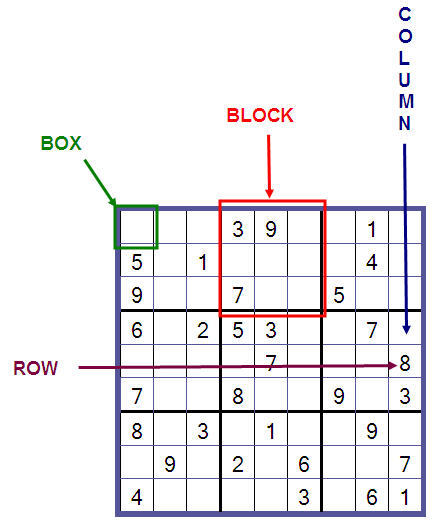
\includegraphics[scale=.5]{sudoku_with_rules.jpg}
\centering
\end{figure}
Previous work has been done to show that solving sudoku puzzles is a binary integer linear programming problem \cite{sudoku3}. With this project, I seek verify through implementation that binary integer programming is applicable to solving different variations of sudoku puzzles.  I also wish to better explain how binary integer linear programming works when being used to solve sudoku puzzles.

\section{Problem Formulation}
\subsection{Model of the Sudoku Puzzle}
It has been shown that binary integer linear programming can be used to solve sudoku puzzles but it is not obvious how this works.  You can think of 9x9 sudoku puzzle as having 9 rows and 9 columns.  If we are at we are the box in the 8,9 position, we are looking at a box that is in the 8th row at the 9th column.
\begin{figure}[H]
\centering
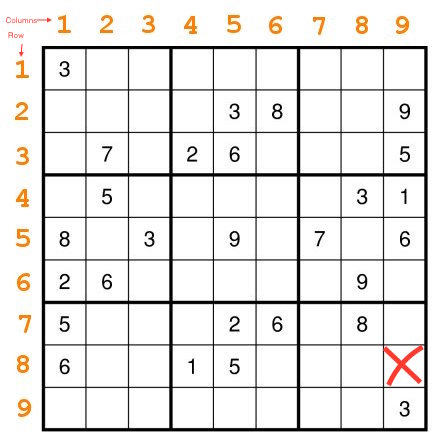
\includegraphics[scale=.4]{sudoku_rows_columns.jpg}
\caption{A red X marks the 8,9 position in the sudoku puzzle.}
\end{figure}
You can then think of each i,j box position in the sudoku puzzle as having a vector of 1's or 0's \cite{sudoku4}.  The size of the vector is the number of possible digits the sudoku puzzle can have.  For example, a 9x9 puzzle has 9 possible digits 1 - 9 that could be in the puzzle so the vector at each i,j position would be of size 9. If the box at 8,8 position had the digit 2 in it then there would be a 1 in the 2nd index of the vector and all other positions would be 0.
\begin{figure}[H]
\centering
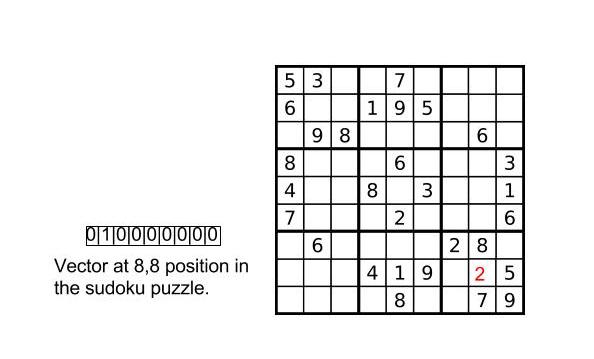
\includegraphics[scale=.4]{sudoku_puzzle_vector.jpg}
\caption{Digit 2 at 8,8 position in the sudoku puzzle.}
\end{figure}
If we let $p$ represent the entire puzzle, we can say that $p_{8,8}$ represents the vector at the 8,8 position of the puzzle.  We can then say $p_{8,8,2}$ represents the value at index 2 of the vector of the box at the 8,8 position in the puzzle which, from figure 2, would be 1.

\subsection{Model of the Sudoku Problem}
Using the model of the sudoku puzzle above, we can formulate a binary integer linear program that will solve the sudoku problem which is made up of the sudoku puzzle and the rules.  We can think of the decision variables of the binary integer sudoku problem as \cite{sudoku4}
\[p_{i,j,k} = 
\begin{cases}
1 \text{ if the i,j position in the puzzle has the value k} \\
0 \text{ if the i,j position in the puzzle does not have the value k} \\
\end{cases}
\]
The decision variables are the digits in each box of the puzzle.  Each decision variable takes on either a 1 or 0 if the digit is supposed to be in the box or not.  This means there are k decision variables for each box at the i,j position in the sudoku puzzle.  For a 9x9 puzzle there are 9x9x9 = 729 decision variables where the number of rows, columns, and digits are all equal to 9.

Given these decision variables we can write the rules of the sudoku problem---there being only one instance of each digit in each row, column, and submatrix (block)---as linear programming constraints.

To model the rule that there is only one instance of each digit in each row we could write the following constraint:
\[
\sum_{j=1}^{n} p_{i,j,k} = 1 \text{  for } i=1...m \text{ and } k=1...z
\]
This says that for each row $i$ and for each digit $k$ in row $i$ there will only be only one instance of the digit $k$ in all of the columns $j$ in that row \cite{sudoku1}.

To model the rule that there is only one instance of each digit in each column we could write the following constraint:
\[
\sum_{i=1}^{m} p_{i,j,k} = 1 \text{  for } j=1...n \text{ and } k=1...z
\]
This says that for each column $j$ and for each digit $k$ in column $j$ there will be only one instance of the digit $k$ in all of the rows $i$ in that column \cite{sudoku1}.

To model the rule that there is only one instance of each digit in each submatrix (block) we could write the following constraints:
\[
\sum_{i=1}^{3} \sum_{j=1}^{3} p_{i+o,j+q,k} = 1 \text{  for } o,q = \{0,3,6\} \text{ and } k = 1...z 
\]
This says there is only one instance of each digit in each of the submatrices (blocks) in the puzzle \cite{sudoku2}.

To model the rule that there has to be at lease one instance of each digit in each box in the sudoku puzzle we could write the following constraints:
\[
\sum_{k=1}^{z} p_{i,j,k} = 1 \text{  for } i = 1...m \text{ and } j = 1...n
\]
This says that for each row $i$ and each column $j$ there is at lease one value $k$ equal to one \cite{sudoku1}.

Finally, to model the given digits in the puzzle we could write the following constraint:
\[
p_{i,j,k} = 1 \text{  for all } i,j,k \text{ in the given puzzle if $k$ is a digit 1...$z$}
\]
This says that we set the digit k at the i,j position in the sudoku puzzle to be 1 if that digit k exists at the i,j position in the given puzzle \cite{sudoku1}.

The sudoku problem is a feasibility problem: we just want to find a solution that produces decision variables (digits) that follow the sudoku rules \cite{sudoku1}.  Therefore, it is not important if the objective function is set to maximize or minimize.

\subsection{Model of Sudoku in Matlab}
Coding the sudoku solver is somewhat more difficult than writing out the constraint equations.  You can use the "intlinprog" function from Matlab and set all of the decision variables as integers to solve a binary integer program for feasibility, but the questions is how do you model the puzzle, the decision variables, and the constraints in matlab.

Code provided by Mathworks, Inc. helped with this process \cite{sudoku2}.  The constraints are modeled as a 3-dimensional array where (1,1,1) matches row 1, column 1, and digit 1.  Coefficients are set to 1 if the constraint is active.  For instance if we were modelling the rule of only one instance of each digit in row 1, we would set all of the coefficients of the columns in row 1 equal to 1 for all of the decision variables (digits).
\begin{figure}[H]
\centering
  \subfloat{
  \includegraphics[scale=.4]{row_constraints.jpg}
  }
  \subfloat{
  \includegraphics[scale=.4]{column_constraints.jpg}
  }
  \subfloat{
  \includegraphics[scale=.4]{submatrix_constraints.jpg}
  }
 \caption{Row 1, column 1, and submatrix 1 (block) constraints in the constraint matrix for digit 1 in Matlab.}
\end{figure}

It is up to "intlinprog" to determine which decision variables (digits) are 1 or 0 for each column in row 1.  This kind of constraint modelling is done for each of the sudoku rules.  Each constraint is appended to the binary linear programming constraint matrix so that it is applied separately from the other constraints to the problem.

The lower bounds for the decision variables are all 0's and the upper bounds are all 1's except for the given digits in the sudoku puzzle.  In that case we set the lower bounds to 1 so that we force the given digits to be 1 in the puzzle so that they must be part of the solution.

Finally, when we do get a solution for the decision variables we must create a 3-dimensional array of 1's and 0's out of the 1-dimensional vector of solutions variables.  We then convert that 3-dimensional array into something that resembles a sudoku puzzle solution.  This is done by multiplying the 1's by their respective digit value and then collapsing the 3-dimensional array into a 2-dimenstional puzzle that can be drawn into a picture of a sudoku puzzle with solutions.

I used and modified the code provided by Mathworks, Inc. to solve 9x9 sudoku puzzles and other variations mentioned in the conclusion of this report.

\section{Conclusion}
\subsection{Sudoku Variations}
Not only can binary integer programming be used to solve 9x9 puzzles but it can be used to solve any kind of variation of sudoku puzzles \cite{sudoku3}.  The variations must satisfy the original constraints and some additional constraint.  In a 16x16 puzzle you have more digits and larger columns, rows, and submatrices (blocks).  
\begin{figure}[H]
\centering
\includegraphics[scale=.5]{16sudoku.jpg}
\caption{An 16x16 sudoku puzzle.}
\end{figure}
In X sudoku you have diagonal lines that must only contain one instance of each digit.
\begin{figure}[H]
\centering
\includegraphics[scale=.5]{sudokuX.jpg}
\caption{An X sudoku puzzle.}
\end{figure}
In 4 Squares sudoku you have 4 additional squares that can only contain one instance of each digit.
\begin{figure}[H]
\centering
\includegraphics[scale=.2]{4squares_sudoku.jpg}
\caption{A 4 Squares sudoku puzzle.}
\end{figure}
Each of these puzzles' rules can be modelled as binary integer linear programming constraints.  This is shown in the implementation part of this project.  What is not shown is how to create sudoku puzzles which is another project in and of itself.

\subsection{Solving Sudoku is NP-Complete}
Finding solution to a Sudoku puzzle is NP-Complete \cite{sudoku3}: no known algorithm exists to solve all sudoku puzzles in polynomial time \cite{sudoku5}.  For a 9x9 puzzle with 27 given digits, to find a solution a solver would at most need to try and check $9^{81-27}$ different matrices.  This, in the worst case, is a exponential runtime \cite{sudoku6}.  Although, once you have a solution you can check it in polynomial time by iterating through the solution matrix and checking it against the constraints.  For a 9x9 puzzle this will take $81^3$ steps: 81 for the row constraints, 81 for the column constraints, and 81 for the submatrix (block) constraints. 

\begin{thebibliography}{1}
\bibitem{sudoku3}
A. C. Bartlett et al., "An Integer Programming Model for the Sudoku Problem", 2008.
\bibitem{sudoku}
T. Hürlimann, "The Sudoku Game I (sudoku)", in \emph{Puzzles and Games: A Mathematical Modeling Approach}, 4th ed., 2016, ch. 5, pp 285-290.
\bibitem{sudoku4}
J. Z. Kolter, "15-780 - Mixed integer programming", 2014.
\bibitem{sudoku1}
W. Olszowy, "Solving sudoku as an Integer Programming problem".
\bibitem{sudoku6}
"Puzzling Computers A gentle introduction to the theory of NP-Completeness.", Available: \url{https://geevi.github.io/2014/puzzles.html}
\bibitem{sudoku5}
\emph{The Math Behind Sudoku} [Online].  Cornell University Department of Mathematics.  Available: \url{http://www.math.cornell.edu/~mec/Summer2009/Mahmood/More.html}
\bibitem{sudoku2}
\emph{Solve Sudoku Puzzles Via Integer Programming} [Online]. The MathWorks, Inc. Available: \url{https://www.mathworks.com/help/optim/ug/solve-sudoku-puzzles-via-integer-programming.html}
\end{thebibliography}

\end{document}
